
\begin{frame}{Motivation: Autonomous driving}

  \begin{tikzpicture}
    \node [anchor=north west,inner sep=0] (img) at (0,0) 
    {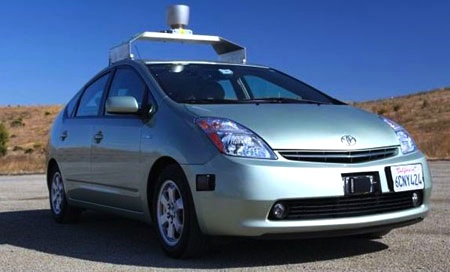
\includegraphics[width=0.42\textwidth, trim=4cm 00cm 1cm 0cm,clip]{graphics/google-laser-scan-cost.jpg}};
    \begin{scope}[x=(img.north east),y=(img.south west)] 
      \coordinate (velc) at (0.25, 0.10);
      \draw [very thick,red] (velc) ellipse (0.25 and 0.10);
      %\draw [->,red] (0,0) -- (1, 0) node {X};
      %\draw [->,red] (0,0) -- (0, 1) node {Y};
    \end{scope}
  \end{tikzpicture}
  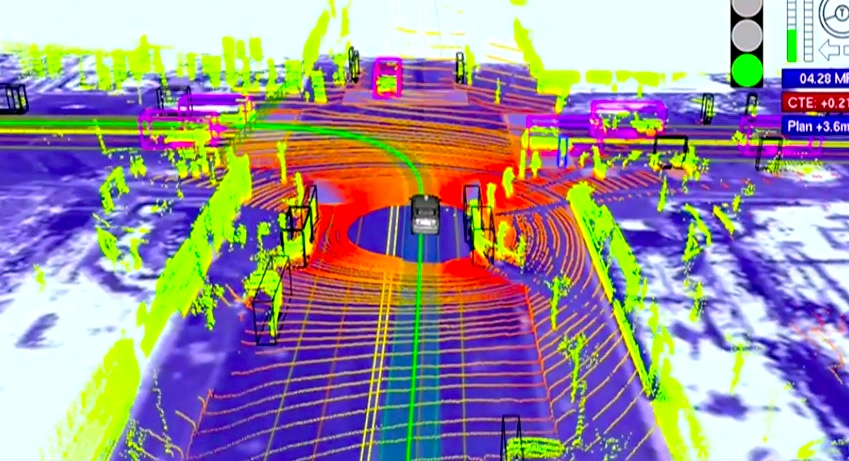
\includegraphics[width=0.50\textwidth, trim=3cm 00cm 3cm 0cm,clip]{graphics/google-laser-scan.jpg}
  \pause

  But Velodyne costs \tikz[remember picture] \node [anchor=north,inner sep=0] (cost) at (0,0) {\$75k};
\end{frame}

\begin{frame}{Can we do it with cameras? Stereo or Monocular}
  \begin{columns}
    \begin{column}{0.48\textwidth}
      \centering
      Left Camera\\
      \includemedia[label=stereoleft,
        width=\textwidth,
        activate=pageopen,
        addresource=graphics/upto61_quat.mp4,
        flashvars={
          source=graphics/upto61_quat.mp4
          &autoPlay=true
          &loop=true             % loop video
          &scaleMode=letterbox   % preserve aspect ratio while scaling the video
        }
      ]{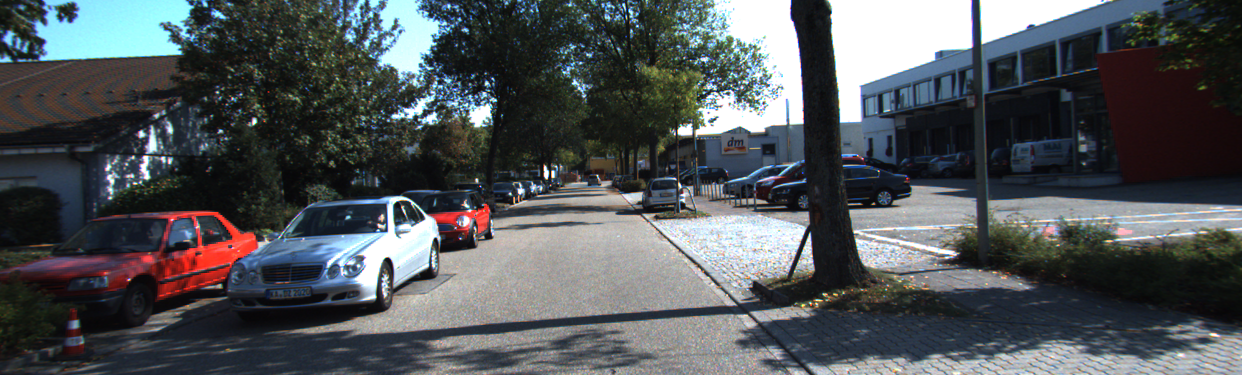
\includegraphics{graphics/0000000061_raw.png}}{VPlayer.swf}
    \end{column}
    \begin{column}{0.48\textwidth}
      \centering
      Right Camera\\
      \includemedia[label=stereoright,
        width=\textwidth,
        activate=pageopen,
        addresource=graphics/upto61_quat_right.mp4,
        flashvars={
          source=graphics/upto61_quat_right.mp4
          &autoPlay=true
          &loop=true             % loop video
          &scaleMode=letterbox   % preserve aspect ratio while scaling the video
        }
      ]{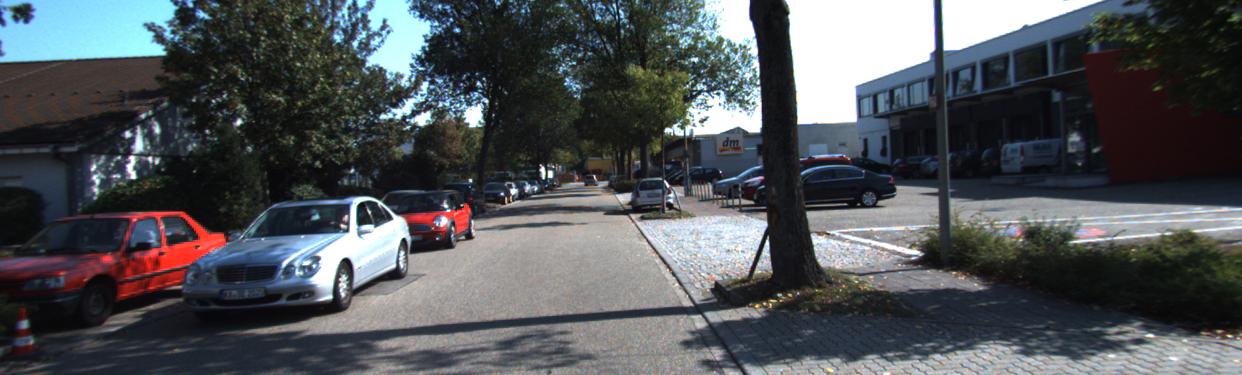
\includegraphics{graphics/0000000061_right.png}}{VPlayer.swf}
    \end{column}
  \end{columns}

  Stereo cameras need to be recaliberated

  And the depth range of stereo cameras are limited

  So after certain depth stereo is same as monocular
\end{frame}

% \begin{frame}{Problem}
%   % Notes: Spend around 30 sec on this slide
%   \centering
%   \begin{figure}
%     
\begin{tikzpicture}[	venn circle/.style={opacity=0.2,fill=#1,draw}]
  %\path[use as bounding box, draw] (-3*1.618, -3) rectangle (3*1.618, 3);

\path[venn circle=red] (0,0) ellipse (3*1.618 and 3);
\node at (0, 1.5) {Autonomous Driving};
\path[venn circle=blue] (0, -1) ellipse (2*1.618 and 2);
\node at (0, 0) {3D Localization};
\path[venn circle=green] (0, -2) ellipse (1.2* 1.618 and 1);
\node at (0, -2) {Occlusion modeling};
\end{tikzpicture}

%   \end{figure}
% \end{frame}
% This slide doesn't make it clear what problem we are trying to solve?  May be
% the slide that Manmohan made with an example image with cars and detections
% is better

% Should we have introduction slide that highlights our contributions?
% but we should have contributions to highlight them. Contributions are perhaps
% better with positive results but still. I don't think we should have negative
% results as a surprise. (It won't as they would have read the report.)

\begin{frame}{Sample input and output}
  \def\arrow{
    (0,0) -- ++(1,0)
    -- ++(0,1) -- ++(0.3, 0)
    -- ++(-0.8, 1) -- ++(-0.8, -1) -- ++(0.3, 0) -- ++(0, -1) }
    \begin{tikzpicture}
      \node[anchor=south west,inner sep=0] (image) at (0,0)
      {
        \includemedia[label=sampleinput,
          width=\textwidth,
          activate=pageopen,
          addresource=graphics/initonly_half.mp4,
          flashvars={
            source=graphics/initonly_half.mp4
            &autoPlay=true
            &loop=true             % loop video
            &scaleMode=letterbox   % preserve aspect ratio while scaling the video
          }
        ]{
        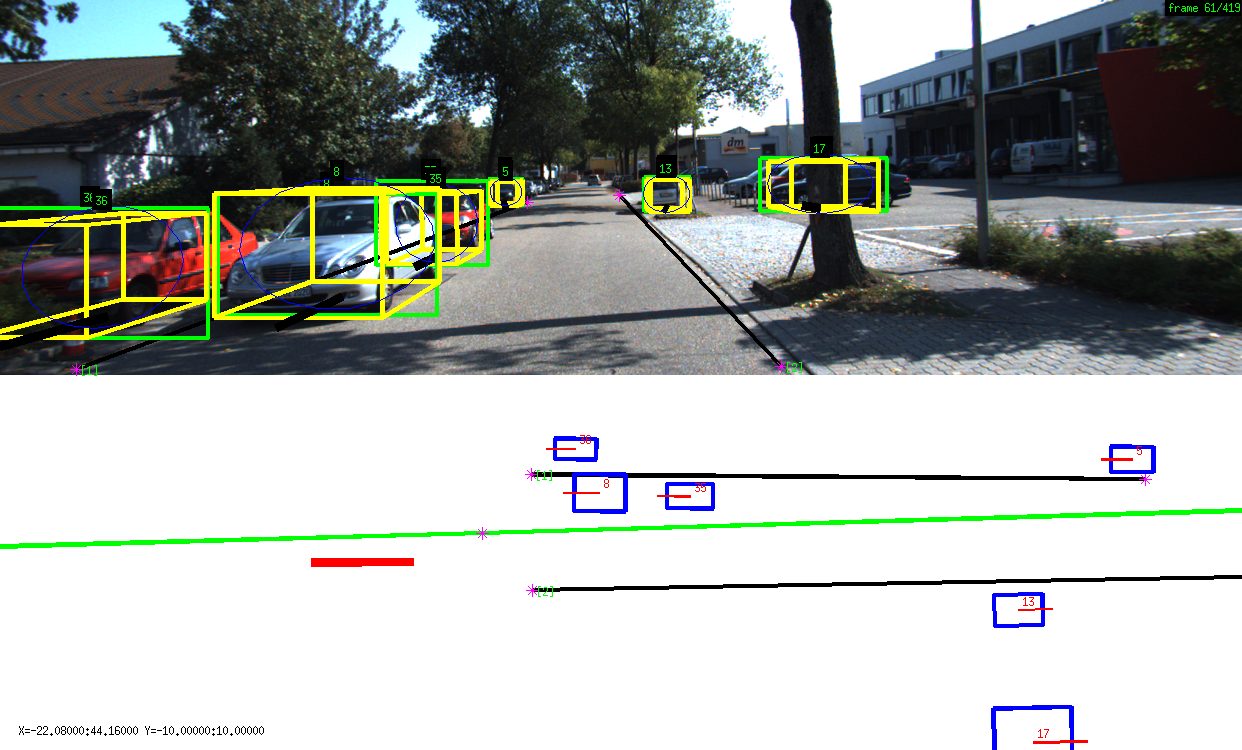
\includegraphics[width=\textwidth]{graphics/0000000061_bevdown.png}    }{VPlayer.swf}
      };
      \begin{scope}[x={(image.south east)},y={(image.north west)}]
        \fill[color=red,scale=0.05,shift={(10,11)},rotate=180,]\arrow;
      \end{scope}
    \end{tikzpicture}

\end{frame}

\begin{frame}{Intermediate inputs}
  % Need a flowchart that describes the input and desired output of the system
 \tikzset{/tikz/x=0.8cm,/tikz/y=0.8cm}
 \setlength{\units}{0.8cm}
  \scriptsize{
    \problemflowchart{}{}{}{}{}
  }
\end{frame}

\begin{frame}{Point tracks example}

  \includemedia[label=pointtracks,
    width=\textwidth,
    activate=pageopen,
    addresource=graphics/pointtracksvideo.mp4,
    flashvars={
      source=graphics/pointtracksvideo.mp4
      &loop=true             % loop video
      &autoPlay=true
      &scaleMode=letterbox   % preserve aspect ratio while scaling the video
    }
  ]{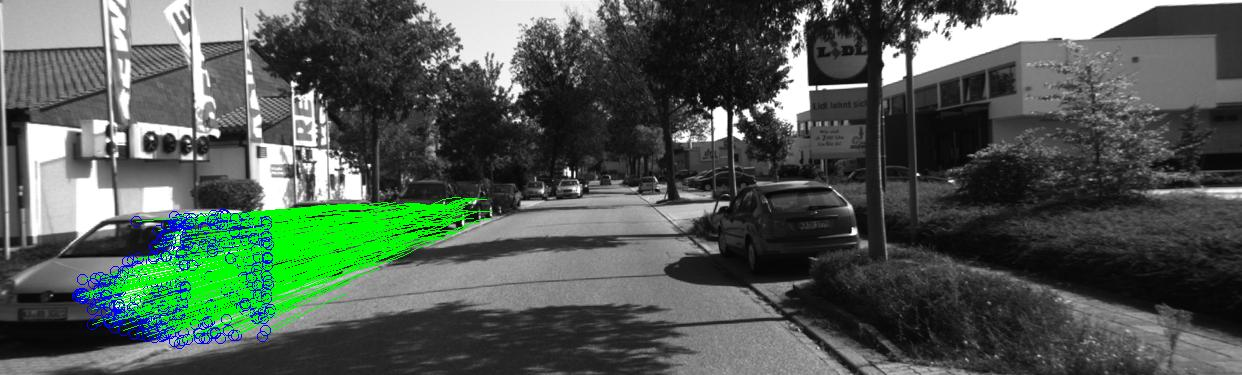
\includegraphics[width=\textwidth]{graphics/object_flow_tracks_4_000033.jpg}}{VPlayer.swf}
\end{frame}

% \begin{frame}{Problem}
%   \visible<-1>{
%     \begin{tikzpicture}
%       \node[anchor=south west,inner sep=0] (image) at (0,0)
%       {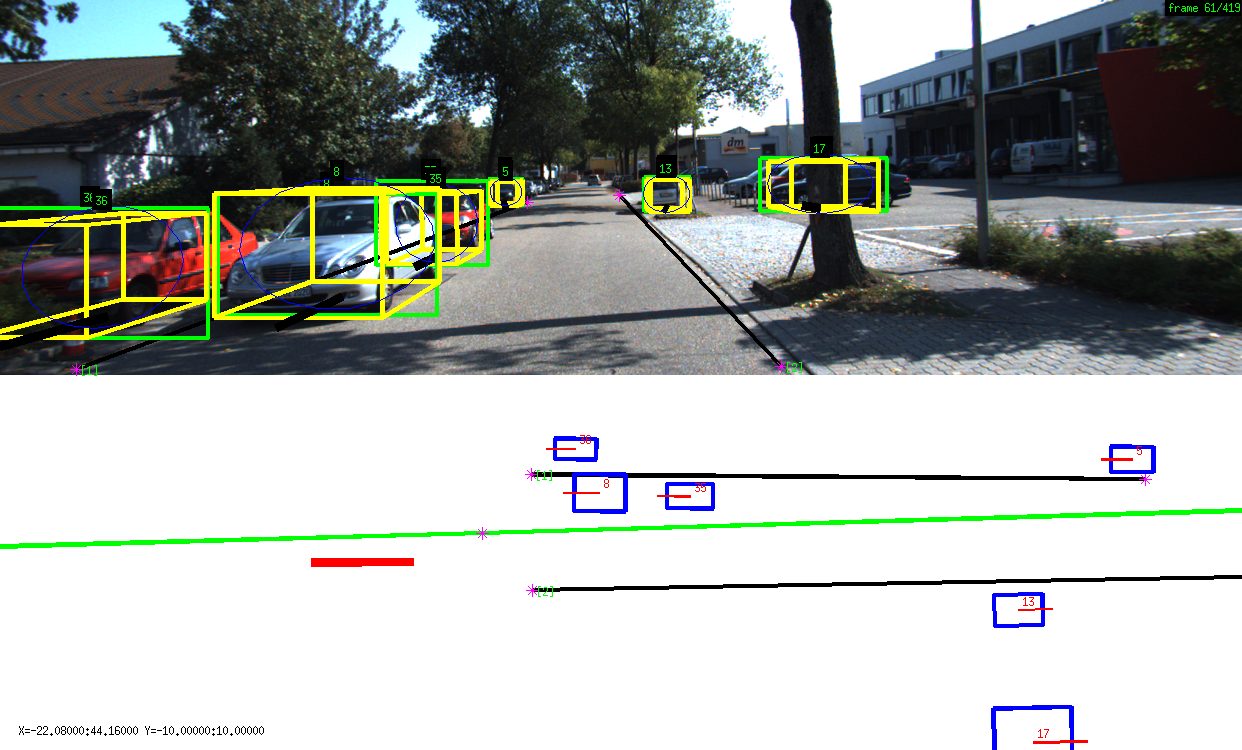
\includegraphics[width=\textwidth]{graphics/0000000061_bevdown.png}};
%       \fill[color=white] (image.south west) rectangle (image.east);
%     \end{tikzpicture}
%   }
% \end{frame}
